\documentclass[final]{beamer}
\mode<presentation>
{
  \usetheme{JDM}
}

\usepackage{multirow}
\usepackage{ragged2e}
\usepackage{times}
\usepackage{amsmath,amssymb}
\usepackage[english]{babel}
\usepackage[latin1]{inputenc}
\usepackage[orientation=landscape, size=custom, width=91, height=114, scale=1]{beamerposter}
\usepackage{array}
\usepackage{xspace}
\usepackage{xcolor}
\usepackage{epsfig}
\usepackage{caption}
\usepackage{subcaption}
\usepackage{booktabs}
\usepackage{wrapfig}

\newcommand{\iqadataset}{\mbox{IQA}}
\newcommand{\thornav}{\mbox{IQA}}

\DeclareMathAlphabet\mathbfcal{OMS}{cmsy}{b}{n}
\newcommand{\model}{$\mathcal{M}$}
\newcommand{\mmodel}{\mathcal{M}}
\newcommand{\visionin}{$\mathcal{V}$}
\newcommand{\mvisionin}{\mathcal{V}}
\newcommand{\languagein}{$\mathcal{L}$}
\newcommand{\mlanguagein}{\mathcal{L}}
\newcommand{\historyin}{$a$}
\newcommand{\mhistoryin}{a}
\newcommand{\mzero}{\textcolor{red}{\vec{0}}}

\newcommand{\navL}{$\mathcal{A}+\mathcal{L}$}  % Navigation No Vision
\newcommand{\navV}{$\mathcal{A}+\mathcal{V}$}  % Navigation No Language
\newcommand{\navA}{$\mathcal{A}$}  % Navigation Action Only
\newcommand{\qaL}{$\mathcal{L}$ \textsc{only}}  % Navigation No Vision
\newcommand{\qaV}{$\mathcal{V}$ \textsc{only}}  % Navigation No Language
\newcommand{\qaA}{$\mathcal{A}$ \textsc{only}}  % Navigation No Language

\newcommand{\good}[1]{\textcolor{blue}{\textbf{#1}}}
\newcommand{\bad}[1]{\textcolor{blue}{\textbf{#1}}}

% Poster text sizes.
\newcommand{\setblocksize}{\LARGE \centering}
\newcommand{\setsize}{\large}
\newcommand{\setcentersize}{\Large}
\newcommand{\paragraphbreak}{\vspace{1cm}}

\title{Shifting the Baseline:\\Single Modality Performance on Visual Navigation \& QA}
\author{Jesse Thomason, Daniel Gordon, and Yonatan Bisk}
\institute{{\texorpdfstring{\color{blue} \bf \large}{ } Jesse Thomason}, Daniel Gordon, and Yonatan Bisk\\University of Washington}

\date{\today}

\begin{document}
\setbeamertemplate{caption}{\raggedright\insertcaption\par}
%%%%%%%%%%%%%%%%%%%%%%%%%%%%%%%%%%%%%%%%%%%%%%%%%%%%%%%%%%%%%%%%%%%%%%%%%%%%%%%%%%%%%%%%%%%
\begin{frame}{} 
  \vfill
  
%\vspace{-270pt}  %added here to get it closer to top...
\begin{columns}[t]

%%%%%%%%%%%%%%%%%%%%%%%%%%%%%%%%%%%%%%%%%%%%%%%%%%%%%%%%%%%%%%%%%%%%%%%%%%%%%%%%%%%%%%%%%%%
\begin{column}{.24\linewidth}    %%% COLUMN 1 %%%

\begin{block}{\setblocksize Why Unimodal Baselines?}
%\vspace{-30pt}
	\vspace{1mm}
\justifying{\setsize
We demonstrate the surprising strength of unimodal baselines in multimodal domains, and make concrete recommendations for best practices in future research.
Where existing work often compares against \textit{random} or \textit{majority class} baselines, 
we argue that unimodal approaches better capture and reflect dataset biases and therefore
provide an important comparison when assessing the performance of multimodal techniques.

}
\end{block}

\begin{block}{\setblocksize Evaluation Framework}
%\vspace{-30pt}
  \vspace{1mm}
\justifying{\setsize

In the visual navigation and egocentric question answering tasks, at each timestep an agent receives an observation and produces an action.
Actions can move the agent to a new location or heading (e.g., \textit{turn left}), or answer questions (e.g., \textit{answer `brown'}).
At timestep $t$, a multimodal model \model{} takes in a visual input \visionin$_t$ and language question or navigation command \languagein{} to predict the next action $a_t$.
The navigation models we examine also take in their own action from the previous timestep, \historyin{}$_{t-1}$, and `minimally sensed' world information $W$ specifying which actions are available (e.g., that \textit{forward} is unavailable if the agent is facing a wall).
\begin{equation}
    a_t \leftarrow \mmodel(\mvisionin_t, \mlanguagein, \mhistoryin_{t-1}; W)
\end{equation} 

We ablate benchmark models from three recent papers:

\begin{enumerate}
\item \textbf{Matterport} Room-2-Room Navigation -- (\textit{Anderson et al., CVPR'18});
\item \textbf{THOR} Interactive Question Answering -- (\textit{Gordon et al., CVPR'18});
\item \textbf{EQA} Embodied Question Answering -- (\textit{Das et al., CVPR'18}).
\end{enumerate}

In each benchmark task, \model{} corresponds to the author's released code and training paradigm.
In addition to their full model, we evaluate the role of each input modality by removing those inputs and replacing them with zero vectors.
Formally, we define the full model and three ablations:

\vspace{-10pt}
\begin{align}
    &\text{Full Model} & \mathrm{is} && \mmodel(\mvisionin_t, \mlanguagein, \mhistoryin_{t-1}; W) \\
    &\mathcal{A} & \mathrm{is} && \mmodel(\hspace{3pt}\mzero\hspace{2pt},\hspace{1pt} \mzero\hspace{2pt}, \mhistoryin_{t-1}; W) \\
    &\mathcal{A+V} & \mathrm{is}& & \mmodel(\mvisionin_t,\hspace{1pt} \mzero\hspace{2pt}, \mhistoryin_{t-1}; W)\\
    &\mathcal{A+L} & \mathrm{is}& & \mmodel(\hspace{3pt}\mzero\hspace{2pt}, \mlanguagein, \mhistoryin_{t-1}; W)
\end{align}
corresponding to models with access to $\mathbfcal{A}$ction inputs, $\mathbfcal{V}$ision inputs, and $\mathbfcal{L}$anguage inputs.
These ablations preserve the architecture and number of parameters of \model{} by changing only its inputs.
\paragraphbreak

\begin{figure}[t]
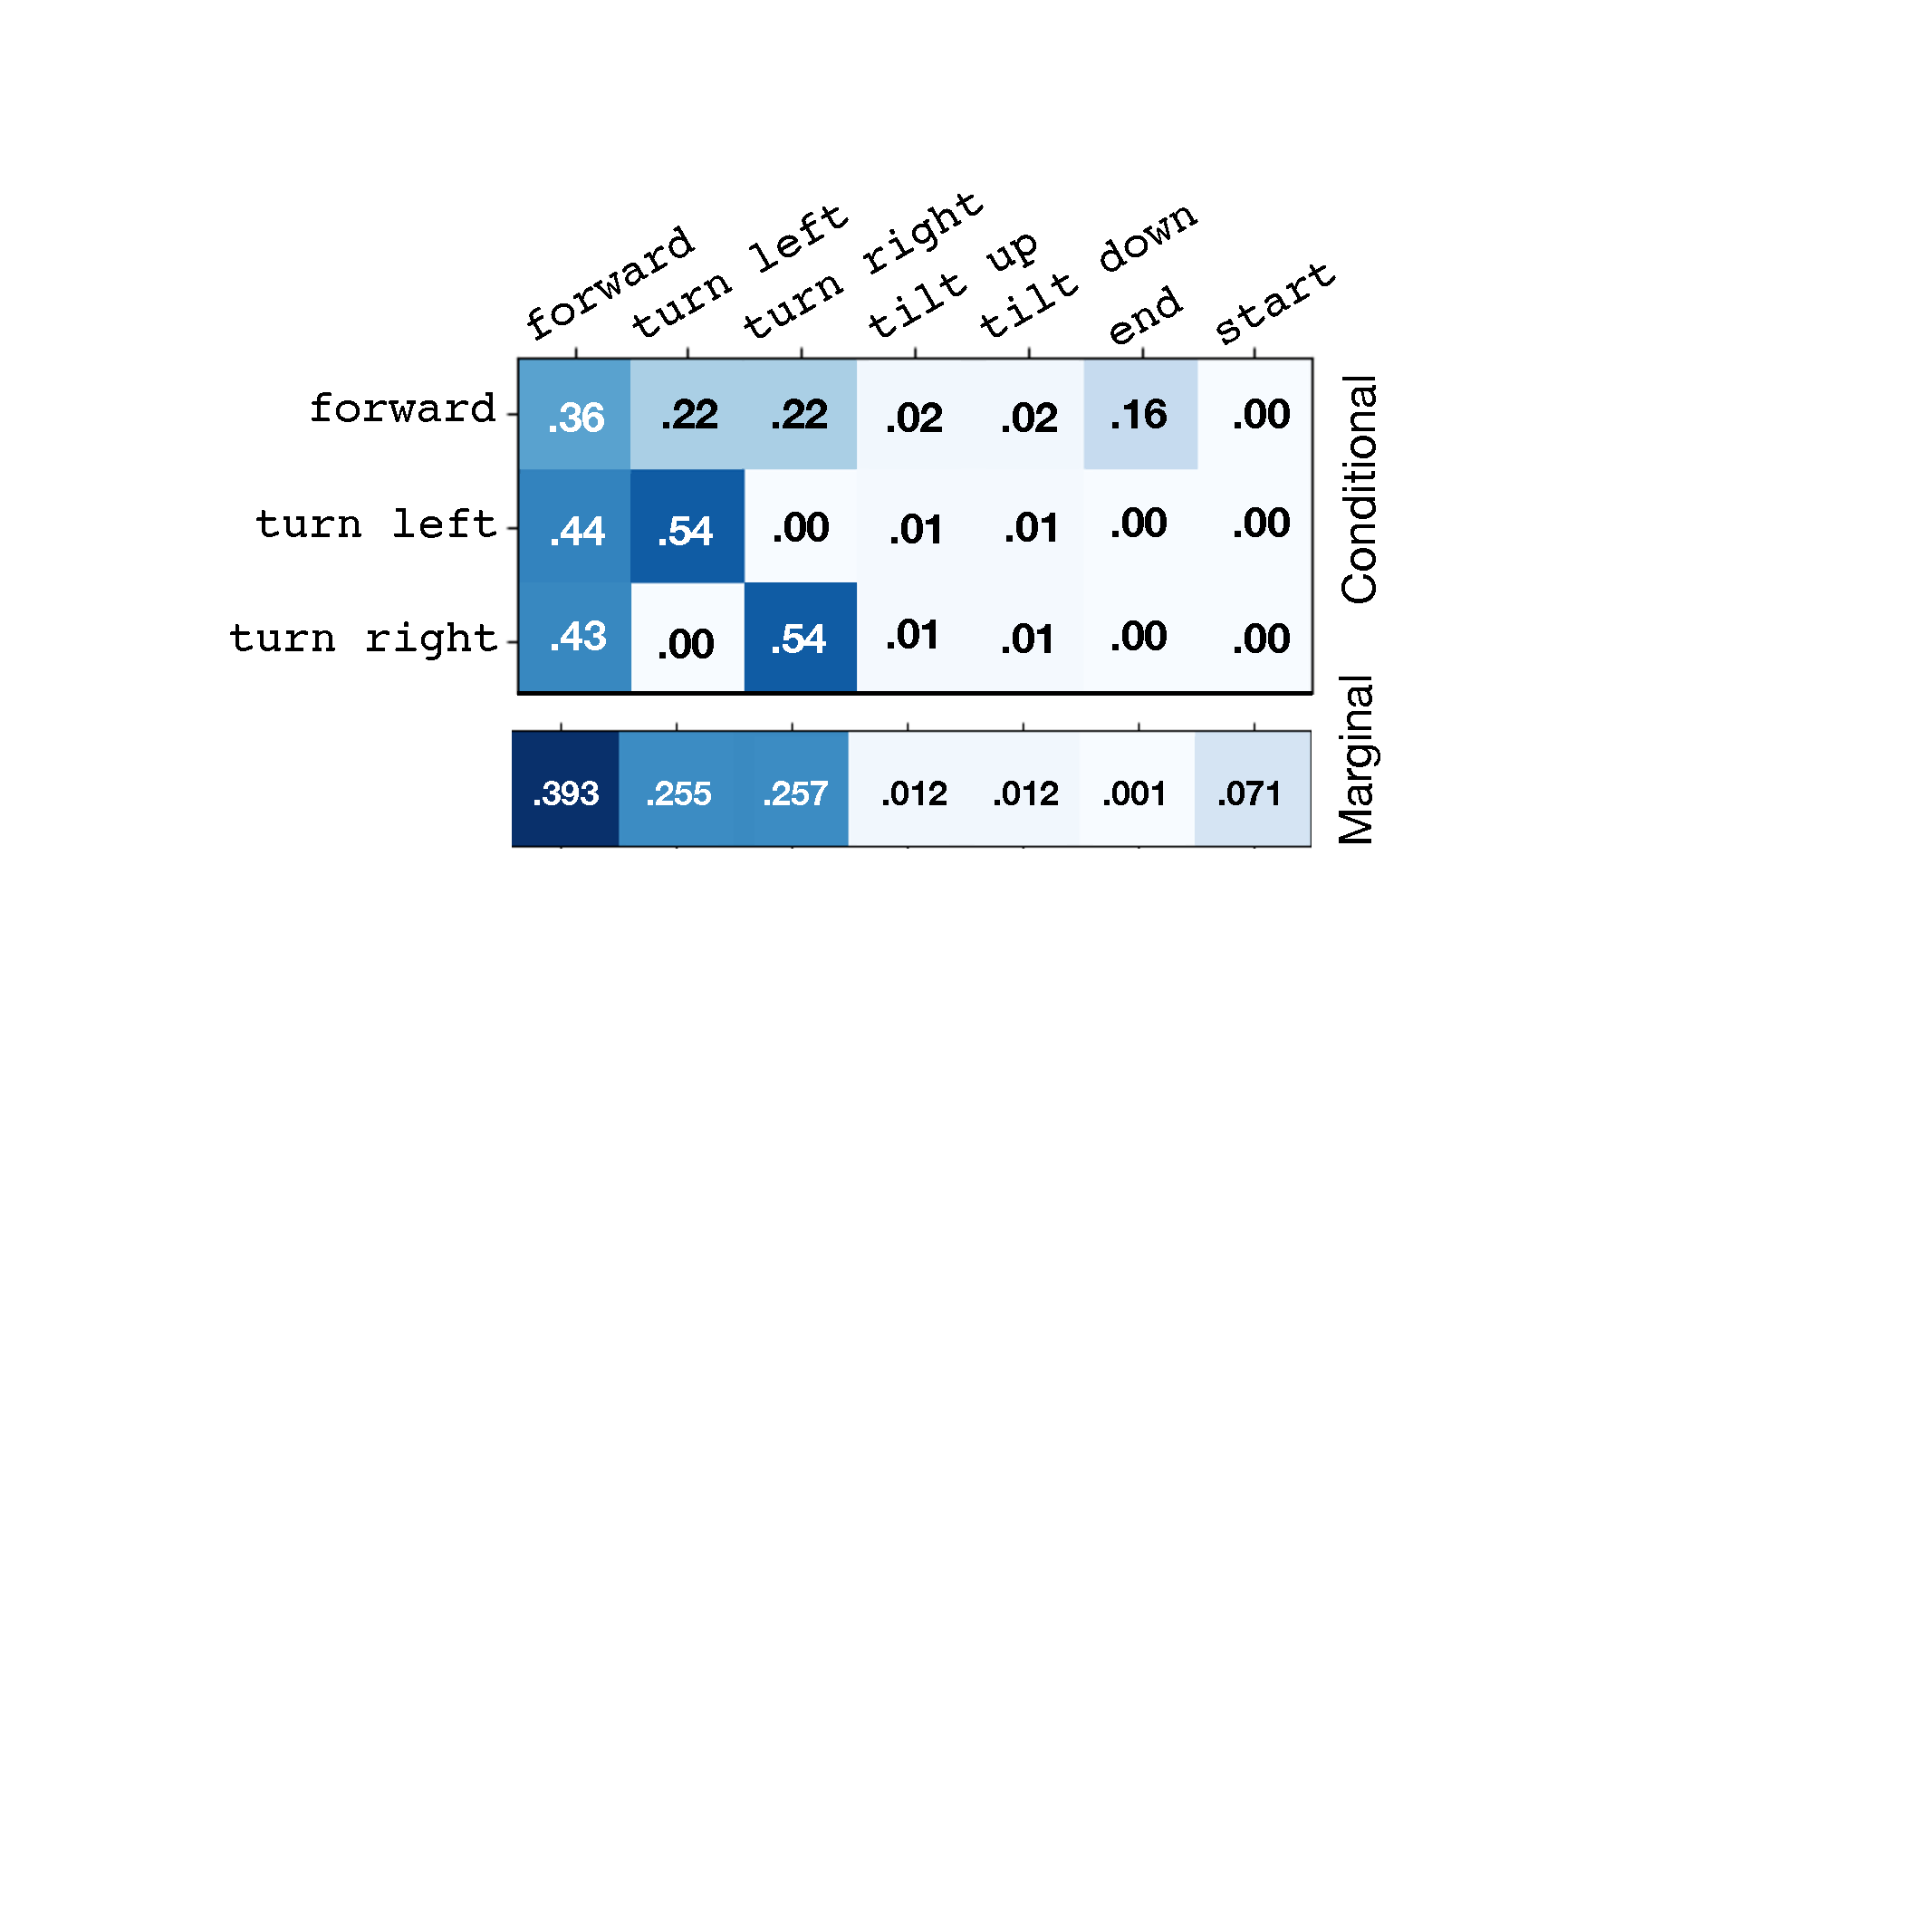
\includegraphics[width=\columnwidth]{figures/matterport_actions_squeeze_top_big.pdf}
\centering
\end{figure}
$P(act=col | prev=row)$ and marginal action distributions in Matterport training data reveal peakiness that enables agents to memorize simple rules like not turning left immediately after turning right, and to move forward an average number of steps.

}
\end{block}

\end{column}	%%% END COLUMN 1 %%%

%%%%%%%%%%%%%%%%%%%%%%%%%%%%%%%%%%%%%%%%%%%%%%%%%%%%%%%%%%%%%%%%%%%%%%%%%%%%%%%%%%%%%%%%%%%
\begin{column}{.49\linewidth}    %%% COLUMN 2 %%%

\begin{block}{\setblocksize }
%\vspace{-30pt}
  \vspace{1mm}
\justifying{\Huge
Language-only and vision-only VLN and QA models outperform published baselines and even beat their multi-modal counterparts.
}
\paragraphbreak

\justifying{\setcentersize
\begin{tabular}{p{650pt}p{150pt}}
\textbf{Recommendation for Best Practices:} Our findings show that in the new space of visual navigation and egocentric QA, all modalities, even an agent's action history, are strongly informative.  Therefore, while many papers ablate either language \textit{or} vision, researchers should ablate \textit{both}.
These unimodal baselines expose possible gains from single-modality biases in multimodal datasets irrespective of training and architecture details. &
\raisebox{-0.9\height}{
\includegraphics[width=0.45\columnwidth]{QR.png}}
\end{tabular}

}
\end{block}

\begin{block}{\setblocksize }
%\vspace{-30pt}
  \vspace{1mm}
\justifying{\setcentersize

\begin{figure}[t]
\centering
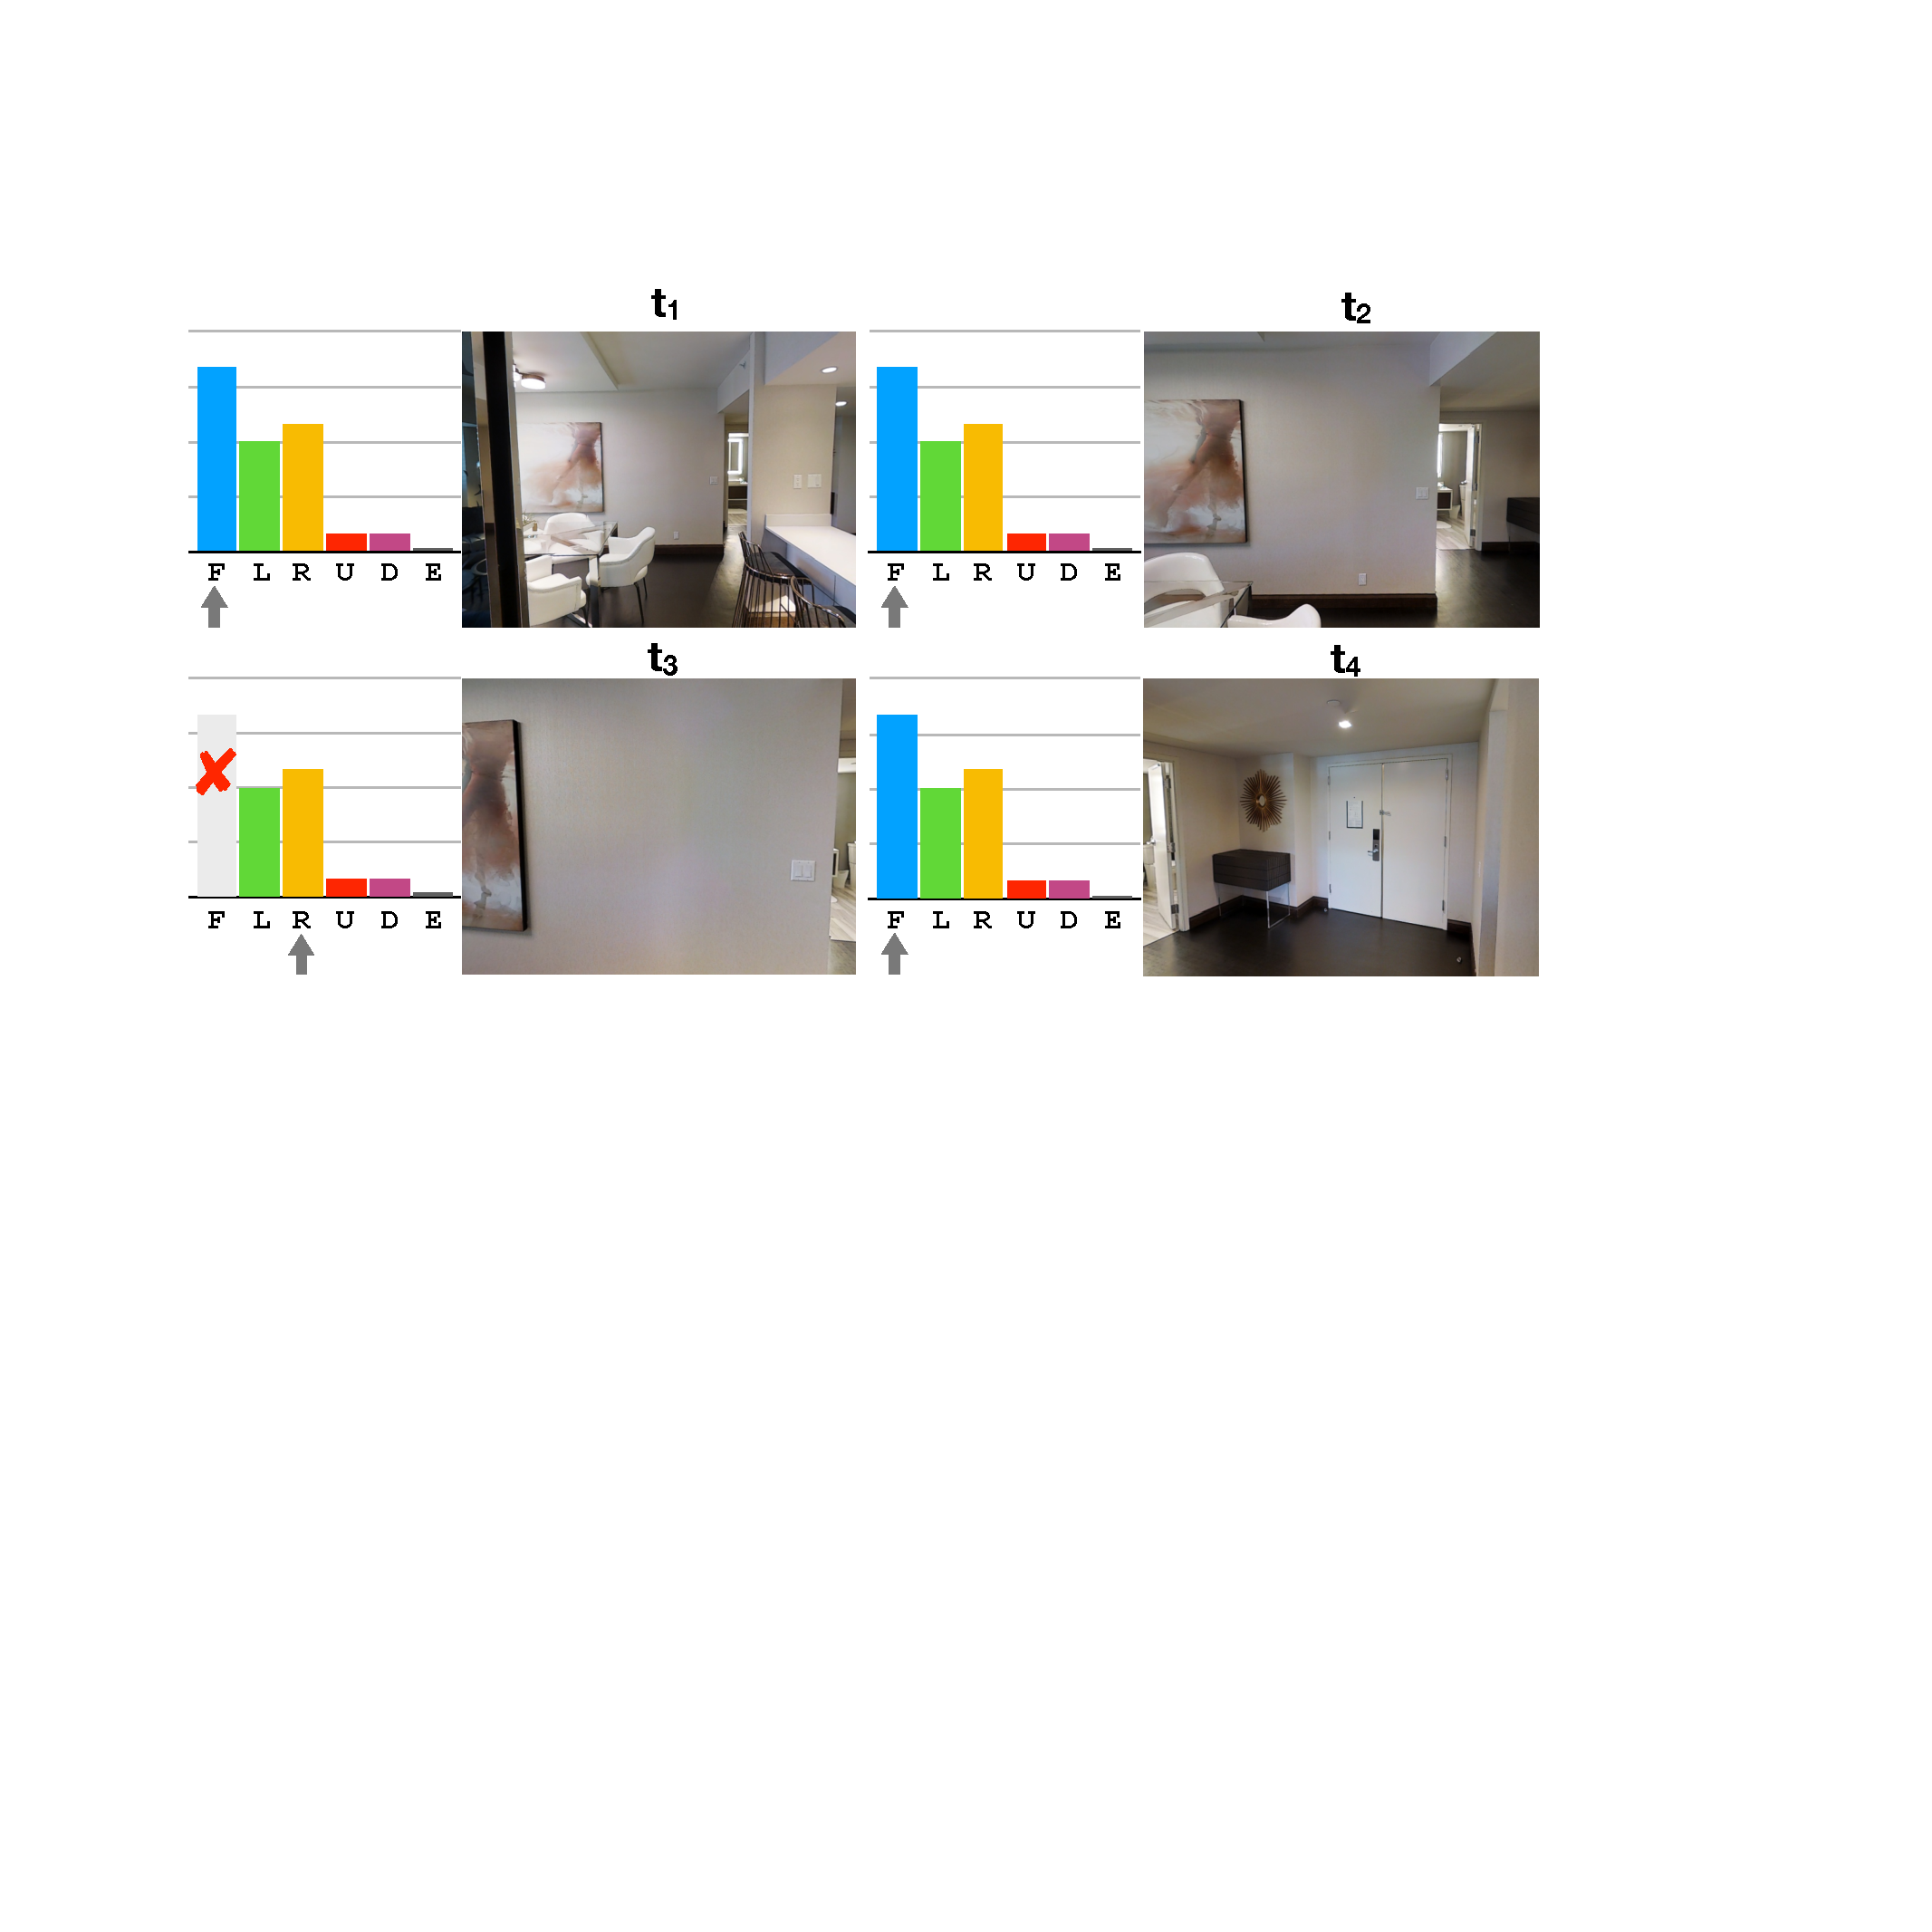
\includegraphics[width=\columnwidth]{figures/Figure1_noLabels.pdf}\\
\vspace{-5pt}\begin{small}Actions: \textbf{\texttt{F}}orward, turn \textbf{\texttt{L}}eft \& \textbf{\texttt{R}}ight, tilt \textbf{\texttt{U}}p \& \textbf{\texttt{D}}own, \textbf{\texttt{E}}nd\end{small}
\end{figure}
In the Matterport Room-2-Room task, navigating without vision can lead to sensible navigation trajectories in response to commands like ``walk past the bar and turn right''.
At $t_3$, ``forward'' is unavailable as the agent would collide with the wall, rendering the visual context for the command unnecessary.
\paragraphbreak

\begin{figure}
\centering
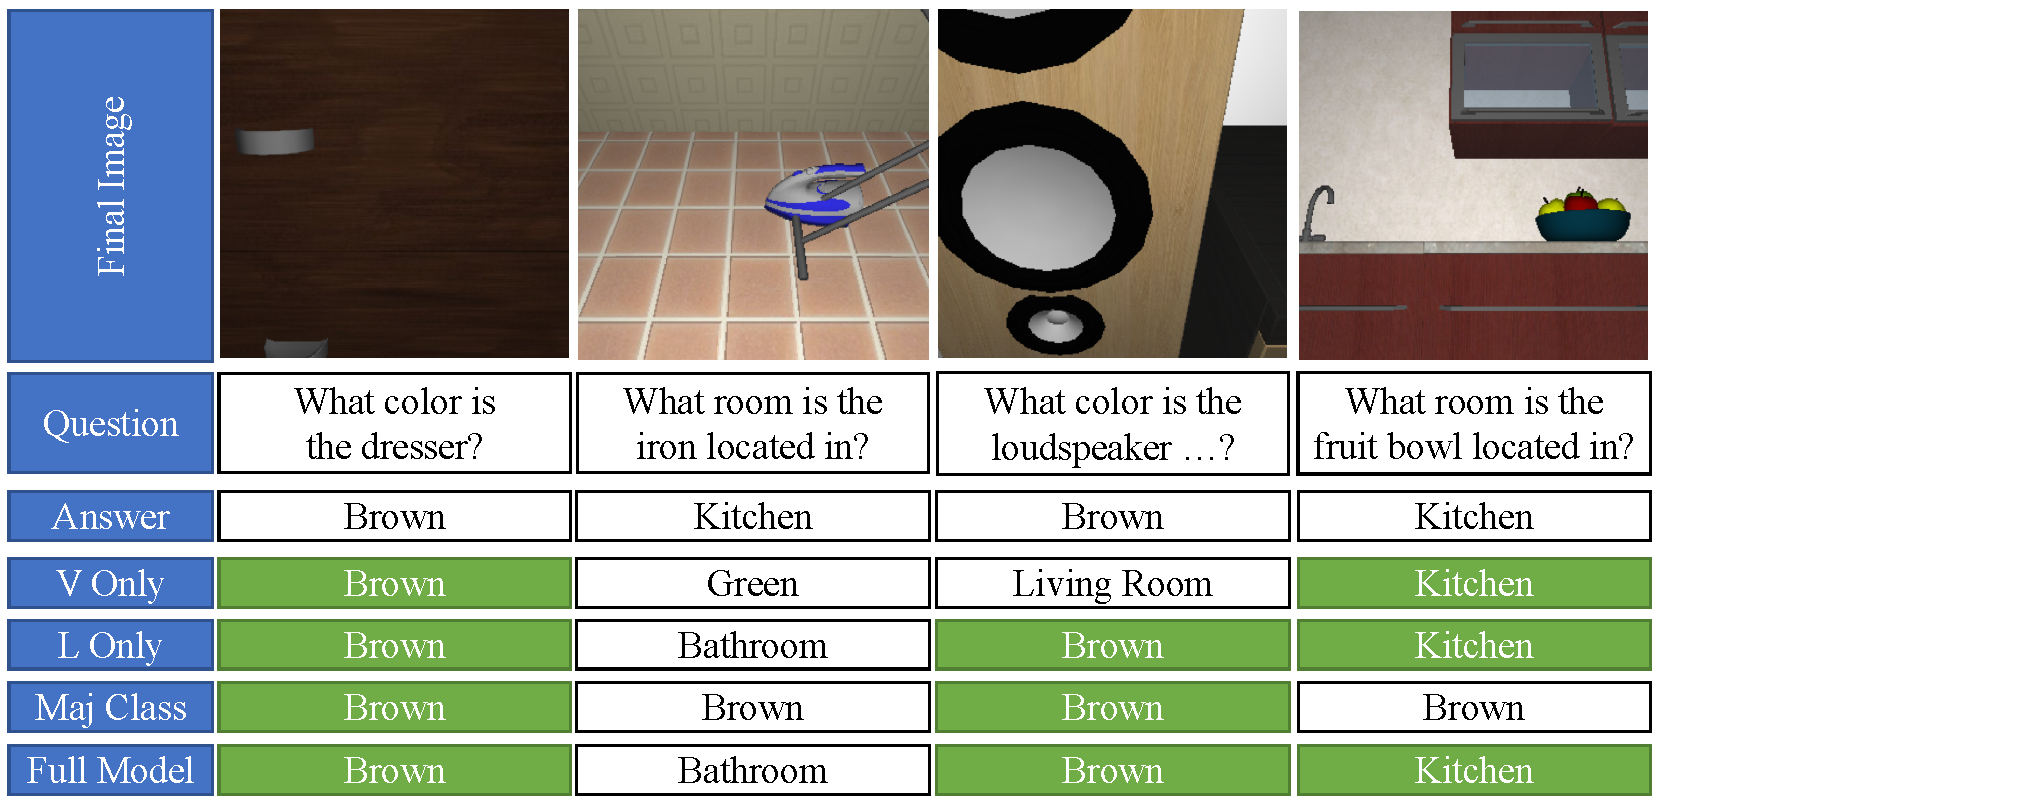
\includegraphics[width=\linewidth]{figures/EQA_samples_1col_4.pdf}
\end{figure}
Qualitative results on the EQA task illuminate some unimodal biases in the data.
The language only model can pick out the most likely answer for a given question without visual context.
The vision only model finds and reports salient color and room feature as answers without being aware of the question.

}
\end{block}

\end{column}  %%% END COLUMN 2 %%%

%%%%%%%%%%%%%%%%%%%%%%%%%%%%%%%%%%%%%%%%%%%%%%%%%%%%%%%%%%%%%%%%%%%%%%%%%%%%%%%%%%%%%%%%%%%
\begin{column}{0.24\linewidth}    %%% COLUMN 3 %%%

\begin{block}{\setblocksize Unimodal Evaluation}
%\vspace{-30pt}
	\vspace{1mm}
\justifying{\setsize

\textbf{Visual Navigation} is evaluated across all three tasks.
Best unimodal ablations are bolded; {\color{blue}blue} indicates better than reported baseline; and $^*$ indicates better than full model.

\begin{table}
\centering
\begin{tabular}{@{}l@{\hspace{5pt}}l@{\hspace{5pt}}r@{\hspace{5pt}}r@{\hspace{13pt}}r@{\hspace{5pt}}r@{\hspace{13pt}}r@{\hspace{0pt}}}
    & & \multicolumn{2}{@{}c@{\hspace{10pt}}}{\textbf{Matterport}$\uparrow$} & \multicolumn{2}{@{}c@{\hspace{10pt}}}{\textbf{\thornav{}}$\uparrow$} & \multicolumn{1}{@{}c@{}}{\textbf{EQA}$\downarrow$}\\
    & & \multicolumn{2}{@{}c@{\hspace{10pt}}}{(\textit{\%})} & \multicolumn{2}{@{}c@{\hspace{10pt}}}{(\textit{\%})} & \multicolumn{1}{@{}c@{}}{ (\textit{m})}\\
    & \textbf{Model} & \textbf{Seen} & \textbf{Un} & \textbf{Seen} & \textbf{Un} &  \textbf{Un}\\
    \toprule
  \multirow{2}{*}{\rotatebox[origin=c]{90}{Pub.}} & Full Model & 27.1 & 19.6 & 77.7 & 18.08 & 4.17 \\ 
  & Baseline & 15.9 & 16.3 & \phantom{0}2.18 & \phantom{0}1.54 & 4.21 \\
  \cmidrule{2-7}
  \multirow{3}{*}{\rotatebox[origin=c]{90}{Uni}} 
  & \navA & 18.5 & 17.1 & \phantom{0}4.53 & \phantom{0}2.88 & 4.53  \\ 
  & \navV & 21.2 & 16.6 & \textbf{\phantom{0}35.6}  & \textbf{\phantom{0}7.50} & \textbf{$^*$4.11} \\
  & \navL & \textbf{23.0} & $^*$\textbf{22.1} & \phantom{0}4.03 & \phantom{0}3.46 & 4.64 \\
  \cmidrule[1pt]{1-7}
  $\Delta$ & Uni --  Base & \bad{\phantom{0}+7.1} & \bad{\phantom{0}+5.8} & \bad{+33.4} & \bad{\phantom{0}+5.96} & \bad{\phantom{0}-0.10} \\
  \bottomrule
\end{tabular}
\end{table}
Trained via behavior cloning, unimodal ablations outperform published baselines in all cases and full models for Matterport and EQA.

\begin{table}
\centering
\begin{tabular}{@{}l@{\hspace{5pt}}l@{\hspace{5pt}}r@{\hspace{5pt}}r@{\hspace{20pt}}}
    & & \multicolumn{2}{@{}c@{}}{\textbf{Matterport}$\uparrow$} \\
    & & \multicolumn{2}{@{}c@{}}{(\textit{\%})} \\
    & \textbf{Model} & \textbf{Seen} & \textbf{Un} \\
    \toprule
    \multirow{2}{*}{\rotatebox[origin=c]{90}{Pub.}} & Full Model & 38.6 & 21.8 \\
  & Baseline   & 15.9 & 16.3 \\
  \cmidrule{2-4}  
  \multirow{3}{*}{\rotatebox[origin=c]{90}{Uni}} & \navA & \phantom{0}4.1 & \phantom{0}3.2 \\ 
  & \navV & \textbf{30.6} & 13.3 \\
  & \navL & 15.4 & \textbf{13.9} \\
  \cmidrule{2-4}
  $\Delta$ & Uni -- Base\phantom{0} & \bad{+14.7} & \phantom{0}-2.4 \\
  \bottomrule
\end{tabular}
\end{table}
Using student forcing, unimodal ablations are no less competitive on unseen environments, but can still memorize seen environments well.

\begin{table}
\centering
\begin{tabular}{@{}l@{\hspace{10pt}}l@{\hspace{10pt}}r@{\hspace{10pt}}r@{\hspace{10pt}}r@{\hspace{10pt}}}
    & & \multicolumn{3}{@{}c@{}}{$\mathbf{d_T}\downarrow$} \\
    & & \multicolumn{3}{@{}c@{}}{(\textit{m})} \\
    & \textbf{Model} & $T_{-10}$ & $T_{-30}$ & $T_{-50}$ \\
    \toprule
  \multirow{2}{*}{\rotatebox[origin=c]{90}{Pub.}} & Full & 0.971 & 4.17 & 8.83 \\
  & Baseline & 1.020 & 4.21 & 8.73 \\ 
  \cmidrule{2-5}
  \multirow{3}{*}{\rotatebox[origin=c]{90}{Uni}} & \navA & \textbf{$^*$0.893} & 4.53 & 9.56 \\ 
  & \navV & $^*$0.951 & \textbf{$^*$4.11} & \textbf{$^{\dagger}$8.83} \\
  & \navL & 0.987 & 4.64 & 9.51 \\
  \cmidrule{2-5}
  $\Delta$ & Uni -- Base\phantom{0} & \bad{-0.127} & \bad{-0.10} & +0.10 \\
  \bottomrule
\end{tabular}

\paragraphbreak

\begin{tabular}{@{}l@{\hspace{10pt}}l@{\hspace{10pt}}r@{\hspace{10pt}}r@{\hspace{10pt}}r@{\hspace{10pt}}}
    & & \multicolumn{3}{@{}c@{}}{$\mathbf{d_{min}}\downarrow$} \\
    & & \multicolumn{3}{@{}c@{}}{(\textit{m})} \\
    & \textbf{Model} & $T_{-10}$ & $T_{-30}$ & $T_{-50}$ \\
    \toprule
  \multirow{2}{*}{\rotatebox[origin=c]{90}{Pub.}} & Full & 0.291 & 2.43 & 6.45 \\
  & Baseline & 0.293 & 2.45 & 6.38 \\ 
  \cmidrule{2-5}
  \multirow{3}{*}{\rotatebox[origin=c]{90}{Uni}} & \navA & $^*$0.242 & 3.16 & 7.99 \\ 
  & \navV & $^*$0.287 & \textbf{2.51} & \textbf{$^*$6.44} \\
  & \navL & \textbf{$^*$0.240} & 3.19 & 7.96 \\
  \cmidrule{2-5}
  $\Delta$ & Uni -- Base\phantom{0} & \bad{-0.053} & +0.06 & +0.06 \\
  \bottomrule
\end{tabular}
\end{table}
EQA navigation across two metrics and three distance settings reveal that, across paradigms, a unimodal ablation can outperform a full model on the task.
\paragraphbreak

\textbf{Question Answering} is evaluated on the IQA and EQA tasks.
\paragraphbreak

\begin{table}
\centering
\begin{tabular}{@{}l@{\hspace{10pt}}lrr@{\hspace{10pt}}r@{\hspace{10pt}}}
    & & \multicolumn{2}{c}{\textbf{\iqadataset{}$\uparrow$}} & \multicolumn{1}{c}{\textbf{EQA $\uparrow$}} \\
    & \textbf{Model} & \textbf{Un} & \textbf{Seen} & \textbf{Un} \\
    \toprule
    \multirow{2}{*}{\rotatebox[origin=c]{90}{Pub.}} & Full Model & \phantom{+}88.3 & \phantom{+}89.3 & \phantom{+}64.0\\ 
     & Baseline & \phantom{+}41.7 &  \phantom{+}41.7 & \phantom{+}19.8 \\
    \cmidrule{2-5}
    \multirow{2}{*}{\rotatebox[origin=c]{90}{Uni}}
    & \qaV & \textbf{\phantom{+}43.5} & \textbf{\phantom{+}42.8} & \phantom{+}44.2 \\
    & \qaL & \phantom{+}41.7 &  \phantom{+}41.7 & \textbf{\phantom{+}48.8} \\
    \cmidrule[1pt]{1-5}
    $\Delta$ & Uni -- Base\phantom{0} & \bad{\phantom{0}+1.8} & \bad{\phantom{0}+1.1} & \bad{+29.0} \\
    \bottomrule
\end{tabular}
\end{table}
In question answering, unimodal ablations outperform published baselines in all cases.
Ablations are not competitive with full models, particularly on the intentionally class-balanced IQA dataset.

}
\end{block}

\end{column}	%%% END COLUMN 3 %%%

%%%%%%%%%%%%%%%%%%%%%%%%%%%%%%%%%%%%%%%%%%%%%%%%%%%%%%%%%%%%%%%%%%%%%%%%%%%%%%%%%%%%%%%%%%%%%%%%%%%%
\end{columns}

\end{frame}

\end{document}


%%%%%%%%%%%%%%%%%%%%%%%%%%%%%%%%%%%%%%%%%%%%%%%%%%%%%%%%%%%%%%%%%%%%%%%%%%%%%%%%%%%%%%%%%%%%%%%%%%%%
%%% Local Variables: 
%%% mode: latex
%%% TeX-PDF-mode: t

